\documentclass[a4paper,11pt,titlepage]{article}
\title{Progetto Basi di Dati\\Gestione di una Palestra durante il Covid-19}
\author{Bit Nicola (878249), Campanelli Alessio (878170), Gottardo Mario (879088)}
\date{AA. 2020/2021}
\pdfpagewidth
\paperwidth
\pdfpageheight
\paperheight
\usepackage[italian]{babel} 
\usepackage{epsfig}
\usepackage{fancyhdr} 
\usepackage{amsmath,amssymb}
\usepackage{amscd} 
\usepackage[T1]{fontenc} 
\usepackage[utf8]{inputenc} 
\usepackage[usenames,dvipsnames]{xcolor}
\usepackage{graphicx,color,listings}
\usepackage{hologo}
\frenchspacing 
\usepackage{geometry}
\usepackage{rotating}
\usepackage{caption}
\captionsetup{labelformat=empty, textfont=sl}
\geometry{a4paper,tmargin=3cm,bmargin=3cm, lmargin=3cm,rmargin=2cm} \usepackage{multirow}
\usepackage{picture}
\usepackage{graphicx}
\graphicspath{{./images/}}
\usepackage{lipsum}  
\newtheorem{theorem}{Theorem}
\textwidth16cm\textheight24cm\topmargin0mm\headheight0mm\headsep6mm\oddsidemargin0mm\evensidemargin0mm

\begin{document}
\maketitle
\tableofcontents
\pagebreak
\section{Introduzione}
Introduzione da scrivere
\subsection{Credenziali di accesso alla rete Hamachi}
\begin{verbatim}
-Nome rete: progetto-DB
-Password: w^JT4fg
\end{verbatim}
\section{Database}
Mamma mia!
\\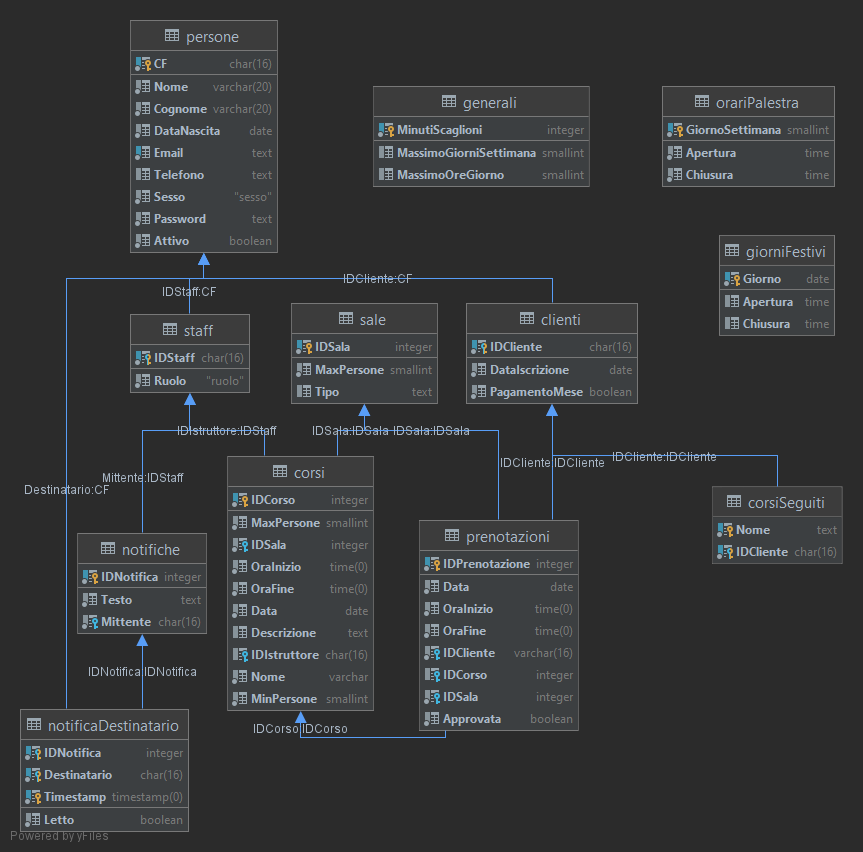
\includegraphics[width=\textwidth]{schema.png}\\
Mamma mia!
\section{Query principali}

\subsection{Contact Tracing}
L'algoritmo di contact tracing prende in ingresso un istanza di Persona che sappiamo essere positiva (da qui in poi "positivo") e un numero di giorni da analizzare (al più 7 per evitare calcoli troppo pesanti), al termine dell'esecuzione, l'algoritmo ritorna una lista di potenziali positivi. L'algoritmo cerca l'ultima data in cui il positivo è entrato nella struttura, determina allora il range usando il numero di giorni in input.\\
Trova tutte le volte in cui il positivo è entrato, per ogni ingresso trova tutte le prenotazioni che intersecano quella in esame e salva il cliente e l'eventuale istruttore nel caso la prenotazione sia riferita ad un corso.
\subsubsection{pseudocodice}
\begin{lstlisting}[language=Python]
def contact_tracing(zero, days):
    potential_infected = [zero.CF]
    days = int(days)
    if days > 7:
        days = 7

    last_zero_appearance_date = ultimo ingresso di positivo nella struttura
    
    if last_zero_appearance_date is not None:
        last_zero_appearance_date = last_zero_appearance_date.Data
    else:
        return [] # Se non e' mai entrato non ci saranno contatti da tracciare
        
    lower_limit_date = last_zero_appearance_date - timedelta(days=days)
    # definiamo il range usando il numero di giorni in input
    
    last_zero_appearances = tutti gli ingressi di positivo nell'intervallo

    for appearance in last_zero_appearances:
        prenotazioni = tutte le prenotazioni che intersecano quella in esame

        if appearance.IDCorso is not None:
            istruttore = istruttore del corso
            potential_infected.append(istruttore)

        for p in prenotazioni:
            potential_infected.append(p.IDCliente)
    return [get_persona_by_cf(cf) for cf in (list(set(potential_infected)))]
    # Ritorniamo l'istanza delle persone il cui codice fiscale risulta tra
    # i potenziali positivi, rimuovendo prima i duplicati
\end{lstlisting}
\subsubsection{Query di contact tracing}
Query per trovare l'ultimo ingresso del paziente zero
\begin{lstlisting}[language=SQL]
SELECT *
FROM prenotazioni p
WHERE p.IDCliente = zero.CF AND p.Data <= CURRENT_DATE AND
 p.Approvata = TRUE
ORDER BY p.DATA DESC
LIMIT 1
\end{lstlisting}

Query per trovare gli ingressi da analizzare del paziente zero
\begin{lstlisting}[language=SQL]
SELECT *
FROM prenotazioni p
WHERE p.IDCliente = zero.CF AND p.Approvata = TRUE AND
	p.Data BETWEEN lower_limit_date AND CURRENT_DATE
ORDER BY p.DATA DESC
\end{lstlisting}

Query per trovare gli ingressi da analizzare del paziente zero
\begin{lstlisting}[language=SQL]
SELECT *
FROM prenotazioni p
WHERE p.IDCliente = zero.CF AND p.Approvata = TRUE AND
	p.Data BETWEEN lower_limit_date AND CURRENT_DATE
ORDER BY p.DATA DESC
\end{lstlisting}


Query per trovare gli ingressi che si sovrappongono a quelli del paziente zero
\begin{lstlisting}[language=SQL]
SELECT *
FROM prenotazioni p
WHERE p.Data  = appearance.Data AND p.IDSala = appearance.IDSala AND
 (p.OraFine >= appearance.OraInizio OR p.OraFine <= appearance.OraFine) 
 AND p.Approvata = TRUE
\end{lstlisting}

\section{Scelte progettuali}

\end{document}